\documentclass[10pt,a4paper]{article} % tamaño de letra y tipo de papel
\usepackage[utf8]{inputenc}
\usepackage[spanish]{babel} % paquete para que reconozca ñ y tildes
\usepackage{amsmath}
\usepackage{upgreek} 
\usepackage{amsfonts}
\usepackage{amssymb}
\usepackage{graphicx} % paquete para incluir imagenes
\graphicspath{ {imagenes/}}
\usepackage[margin=1in,bottom=1in]{geometry}
\usepackage{hyperref} % paquete para tener marcadores en el pdf
\usepackage{tikz}
\usetikzlibrary{babel}
\usepackage[siunitx, RPvoltages]{circuitikz}
\usetikzlibrary{bending,arrows.meta,positioning,calc,positioning}
\usepackage{pgfplots}\pgfplotsset{compat=1.13}

\pgfplotsset{width=12cm,legend style={at={(0.11,0.75)},anchor=south},select coords between index/.style 2 args={
		x filter/.code={
			\ifnum\coordindex<#1\def\pgfmathresult{}\fi
			\ifnum\coordindex>#2\def\pgfmathresult{}\fi
		}
}}
\author{Ulloa Daniel & Rodriguez Victoria}
\begin{document}

\begin{titlepage}
	\hbox{
		\hspace*{0.15\textwidth} % Espacio desde el margen izquierdo
		\rule{1pt}{\textheight} % Linea decorativa
		\hspace*{0.05\textwidth} % Espacio entre la linea y el texto
		\parbox[b]{0.75\textwidth}{ % Caja que restringe el espacio que puede ocupar el texto
			{\noindent\Huge\bfseries Informe de Laboratorio } % Titulo
			\\ 
			[2\baselineskip] 
			{\large \textbf{Tema:} Oscilador con Resistencia Negativa} % Tema
			\\[4\baselineskip]
            {\large \textbf{Cátedra:} Teoría de Circuitos \textsc{II}} % Catedra
            \\[1\baselineskip]
            {\large \textbf{Año:} 2019} % Año
			\\[1\baselineskip]
            {\large \textit{\textbf{Docentes:} % Docentes
                \textnormal{Ing. Costa}, Nicolás. 
                \textnormal{Aux. Consiglio}, Dante}
            }
			\\[1\baselineskip]
            {\large \textit{\textbf{Alumnos:} % Alumnos
                \textnormal{Rodriguez}, Ana Victoria. 
                \textnormal{Ulloa}, Daniel Alejandro}
            }
            \\[6\baselineskip]
            {\large \textbf{Fecha de Entrega:} 11/09/2019}
			\par %Para que el logo aparezca al pie
			\vspace{0.35\textheight} % Ubicacion de la caja desde el margen superior
            \center{
\includegraphics[width=250px]{logo2.png}}
            \\[1\baselineskip]
	}}
\end{titlepage}
\tableofcontents
\newpage
\section{Introducción}
\begin{center}
    \begin{circuitikz}[american voltages,american inductors]
        \draw (0,0) node [op amp](amp){};
        \draw (amp.-) to [C,l=$C$,v_<=$V_{C(0)}$] ++(-2,0) to [L,l=$L$,i>_=$i$] ++(-2,0) to [R,l=$R_1$] ++(-2,0) node[ground]{};
        \draw (amp.-) to[short,*-] ++(0,1.5) coordinate (leftR2) to[R,l=$R_2$] (leftR2 -| amp.out) to[short,-*] (amp.out);
        \draw (amp.out) to [R,l=$R_a$]++(0,-2) coordinate (rightRa);
        \draw (amp.+) to [short]++(0,-1.51) to [short,-*](rightRa) node [right]{};
        \draw (rightRa) to [R,l=$R_b$]++(0,-2) node[ground]{};
        \draw (amp.out) to [short,*-o]++(1,0)node [right] {$V_{o(t)}$};	
        \draw (amp.up) --++(0,0.1) node[vcc]{12\,\textnormal{V}};
        \draw (amp.down) --++(0,-0.1) node[vee]{-12\,\textnormal{V}};
    \end{circuitikz} 
\end{center}


El sistema de la figura lleva el nombre de oscilador con resistencia negativa, por inspección, se puede observar que el circuito es una configuración RLC serie acompañada de un Conversor de Impedancias Negativas:
%conversor imp negativa
\begin{center}
    \begin{circuitikz}[american voltages]
        \draw (0,0) node [op amp](amp){};
        \draw (amp.-) to [short,o-*,f<^=$I_1$]++(-2,0) node [left] {$V_1$};
        \draw (amp.-) to[short,*-] ++(0,1.5) coordinate (leftR2) to[generic,l=$Z$] (leftR2 -| amp.out) to[short,-*] (amp.out);
        \draw (amp.out) to [R,l=$R_2$]++(0,-2) coordinate (rightRa);
        \draw (amp.+) to [short]++(0,-1.51) to [short,-*](rightRa);
        \draw (rightRa) to [R,l=$R_1$]++(0,-2) node[ground]{};
        \draw (amp.out) to [short,*-o]++(1,0)node [right] {$V_2$};
    \end{circuitikz}
\end{center}

La impedancia de entrada de este circuito es $Z_{in}=V_1/I_1$.

\begin{equation*}
%R1=\frac{R2*Rb}{Ra}
\end{equation*}
Si las resistencias $R_1$ y $R_2$ son iguales entonces la impedancia $Z_{in}=-Z$. Por lo tanto se puede representar el circuito de la siguiente manera:

\begin{center}
    \begin{circuitikz}[american voltages,american inductors]
        \draw (0,0) -- (0,-1) node[ground]{}; 
        \draw (0,0) to[R, l=$R_1$] (2,0);
        \draw (2,0) to [L,l=$L_1$,i_<=$i_L$] (4,0);
        \draw (4,0) to [C,l=$C_1$,v_>=$V_{C(0)}$] (6,0);	
        \draw (6,0) to [generic, l=$Z_{in}$] (8,0);
        \draw (8,0) -- (8,-1) node[ground]{};
    \end{circuitikz}
\end{center}

Esta impedancia negativa $Z_{in}$ compensa las pérdidas de energía en la resistencia $R_1$ y como consecuencia el circuito se comporta como un oscilador con frecuencia angular $\frac{1}{\sqrt{LC}}$.

El circuito RLC junto al conversor de impedancia negativas conforman un sistema de segundo orden. El modelo teórico de la función de transferencia se muestra a continuación:
\begin{equation*}
    H(s)=\dfrac{Y(s)}{U(s)}=\dfrac{K}{s^{2}\tau^{2}+2\xi \tau s+1}
\end{equation*}

En los sistemas de segundo orden existen tres parámetros a considerar:
    \begin{itemize} 
    	\item K: ganancia estática
    	\item $\xi$: factor de amortiguamiento
    	\item $1/\tau$: frecuencia natural no amortiguada
    \end{itemize}
       La posición de los polos está determinada por el factor de amortiguamiento, $\xi$. 
       \begin{equation*}
       p_{1,2}=\frac{1}{\tau}\left(-\xi\pm\sqrt{\xi^2-1}\right)
       \end{equation*}
       Para obtener la característica de un oscilador los polos deben ser imaginarios puros, por lo tanto 
       $\xi$ debe ser nula. 
 

\section{Objetivos}
\begin{itemize}
    \item Modelar e interpretar el Circuito
    \item Obtener la respuesta temporal de la tensión de salida y graficarla en Mathematica
    \item Realizar un barrido paramétrico sobre la resistencia $R_B$ y observar las diferentes respuestas.
\end{itemize}

\section{Modelado Matemático}
Para modelar el circuito se tuvieron en cuenta algunas consideraciones
%\begin{center}
%    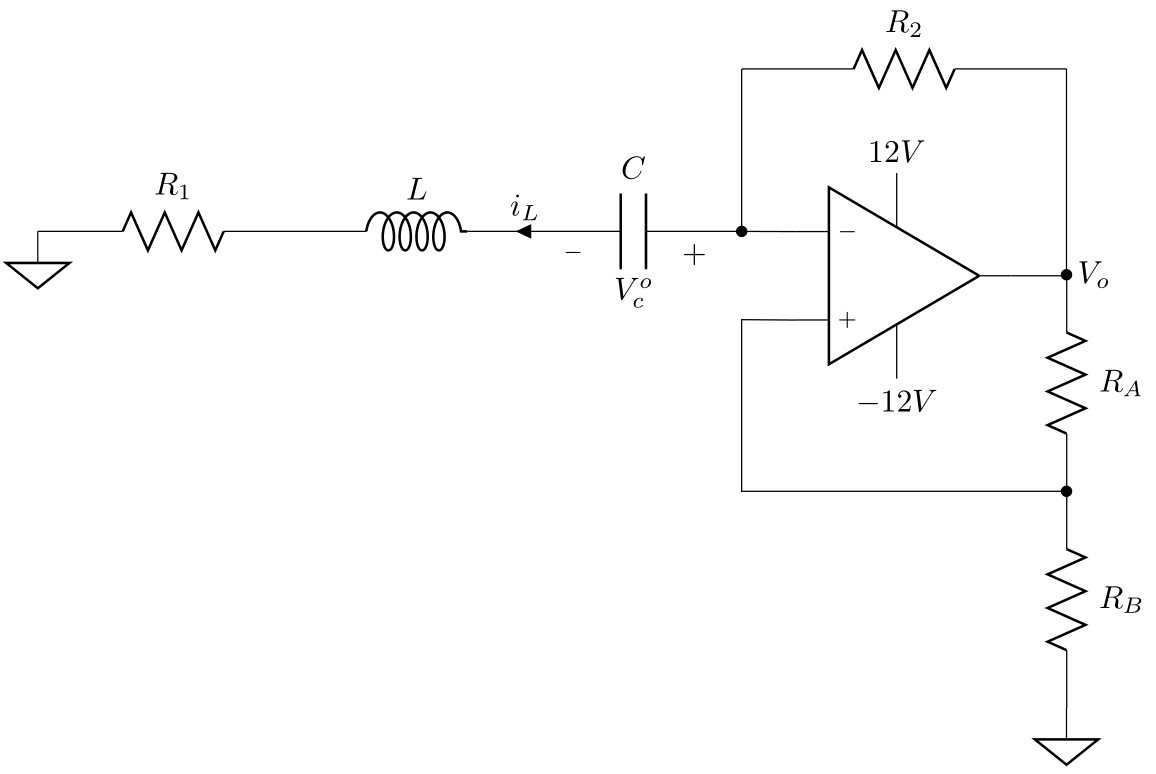
\includegraphics[width=300px]{circuito}
%\end{center}

\begin{itemize}
    \item El amplificador operacional es ideal
    \item La tensión inicial en el capacitor es $V_{C(0)}$
    \item La corriente del capacitor se expresará de forma diferencial
    %\item La corriente en el inductor es la misma que en el capacitor y en las resistencias $R_1$ y $R_2$
    \item La entrada del sistema es la tensión inicial del capacitor
    \item La salida del sistema es la tensión a la salida del Amplificador Operacional
\end{itemize}

\begin{circuitikz}[american voltages,american inductors]
	\draw (0,0) node [op amp](amp){};
	\draw (amp.-) to [C,l=$C$,v_<=$V_{C(0)}$] ++(-2,0) to [smeter, t=A, l=$i\text{=}C\frac{dV}{dt}$]++(-2,0) to [L,l=$L$,i>_=$i$] ++(-2,0) to [R,l=$R_1$] ++(-2,0) node[ground]{};
	\draw (amp.-) to[short,*-] ++(0,1.5) coordinate (leftR2) to[R,l=$R_2$,i<=$i$] (leftR2 -| amp.out) to[short,-*] (amp.out);
	\draw (amp.out) to [R,l=$R_a$]++(0,-2) coordinate (rightRa);
	\draw (amp.+) to [short]++(0,-1.51) to [short,-*](rightRa) node [right] {$V_p$};
	\draw (rightRa) to [R,l=$R_b$]++(0,-2) node[ground]{};
	\draw (amp.out) to [short,*-o]++(1,0)node [right] {$V_{o(t)}$};	
	\draw (amp.up) --++(0,0.1) node[vcc]{12\,\textnormal{V}};
	\draw (amp.down) --++(0,-0.1) node[vee]{-12\,\textnormal{V}};	
\end{circuitikz}
	
Para la primera ecuación se analizó el nodo $V_n$, en donde se tiene que:
\begin{equation*}   
i(t)=i_{R2}(t)
\end{equation*}
Expresando las corrientes de forma diferencial:
\begin{align*}
i(t)&=C\frac{d V_{c}(t)}{dt} \\
i_{R2}(t)&=\frac{V_{o}(t)-V_{n}(t)}{R_{2}} \\
V_{p}(t)&=\frac{R_{b} V_{o}(t)}{R_{a}+R_{b}}
\end{align*}
Donde las tensiones $V_{n}(t)$ y $V_{p}(t)$ son iguales al considerar que el amplificador operacional es ideal.


De esta manera se obtiene la primera ecuación de nuestro sistema, a la cual se le aplicó la transformada de Laplace. 
\begin{equation}
C(s V_{c}(s)-V_{c}(t))-\frac{R_{a} V_{o}(s)}{R_{2} R_{a} +R_{2} R_{b}}=0
\end{equation}
Para la segunda ecuación se analizó la malla que contiene a los componentes $R_{1},\ R_{2},\ C$, $L$ y $V_{o}(s)$ 

\begin{align*}
 V_{o}(t)&=\ V_{C}(t)+ V_{L}(t)+ V_{r}(t)\\
V_{o}(t)&=LC\frac{d V_{c}^{2}(t)}{dt^{2}}+ C(R_{1}+R_{2})\frac{d V_{c}(t)}{dt}+V_{c}(t)
\end{align*}
Nuevamente se aplico la transformada de Laplace, obtiendo la segunda ecuación
\begin{equation}
V_{c}(s) - V_{o}(s) + C(R_{1} + R_{2})(sV_{c}(s) - v_{0}(t)) + 
LC(s^{2}V_{c}(s) - sv_{0}(t)) = 0
\end{equation}
Con estas dos ecuaciones es posible obtener las tensiones de salida y entrada del sistema y su función de transferencia 
\begin{align*}
H(s)&=\frac{C R_{2} (R_{a}+R_{b})}{sR_{a}C (s\text{L} +R_{1}+2 R_{2})-s\text{C}R_{2} R_{b} -R_{a}}\\
H(s)&=\frac{CR_2(R_a+R_b)}{s^2R_aLC+s(CR_2R_b-CR_1Ra)-R_a}
\end{align*}
Reordenando la función de transferencia
\begin{equation*}
H(s)=\frac{-\frac{CR_{2}(R_{a}+R_{b})}{R_{a}}}{-s^{2}(LC)+s(CR_1-\frac{CR_2R_b}{R_a})+1}
\end{equation*}
\\
Comparando la función de transferencia obtenida con la función del modelo teórico se determinaron los parámetros $\xi$, $\tau$ y K
\begin{align*}
K&=-\frac{CR_{2}(R_{a}+R_{b})}{R_{a}}\\
\tau&=\sqrt{LC}\\
\xi&=\dfrac{-CR_{1}+\frac{CR_{2}R_{b}}{R_{a}}}{2\sqrt{LC}}\\
\end{align*}
%despejando la ecuacion anterior para un coeficiente de xi nulo, podemos observar que R1 tiene que ser igual a .... 
%Lo cual coincide con la condición de que para que el circuito se comporte como un oscilador R1 debe estar compesada por la impedancia del conversor de impedancia. 
Un coeficiente de amortiguamiento nulo implica que la resistencia $R_{1}$ debe ser igual a la impedancia vista desde el circuito RLC.
\begin{align*}
\xi&=0\\
R_{1}&=\frac{R_{2}R_{b}}{R_{a}}\\
H(s)&=-\frac{\frac{R_{2}C (R_{a}+R_{b})}{R_{a}}}{\left(LCs^2+1\right)}
\end{align*}
Por último se verificó que los polos están ubicados en el eje imaginario, lo cual cumple con la característica de un oscilador.
 \begin{equation*}
p_{1,2}=i\frac{1}{\sqrt{\text{L}\text{C}}},-i\frac{1}{\sqrt{\text{L}\text{C}}}
\end{equation*}
\section{Respuesta Temporal}
Como vimos anteriormente el valor de $\xi$ determina la ubicación de los polos. Como se fijaron los valores de $R_1$,$R_a$,$R_b$,L y C, el componente que determina la respuesta del sistema es $R_2$.
\begin{center}
	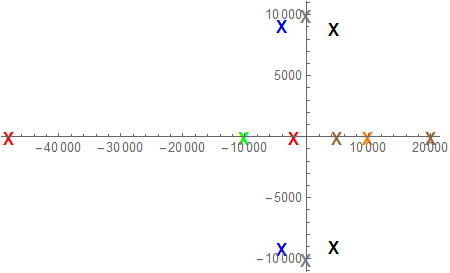
\includegraphics[scale=0.8]{polos1}
\end{center}
\begin{center}
	\begin{tabular}{|c|c|c|}
		\hline 
		Color&$R_{2}$ & Tipo de Respuesta \\ 
		\hline 
		\hline 
		Rojo&500 & Criticamente Amortiguada \\ 
		\hline 
		Verde&800 & Subamortiguada \\ 
		\hline 
		Azul&920 & Sobreamortiguada \\ 
		\hline  
		Gris&1000 &Oscilatoria \\ 
		\hline 
		Negro&1005&Inestable  \\ 
		\hline 
		Naranja&1200&Inestable  \\
		\hline
		Marrón&1250&Inestable  \\
		\hline
	\end{tabular} 
\end{center}

Dados los valores de la tabla para $R_2$ se graficaron las respuestas temporales
\begin{center}
	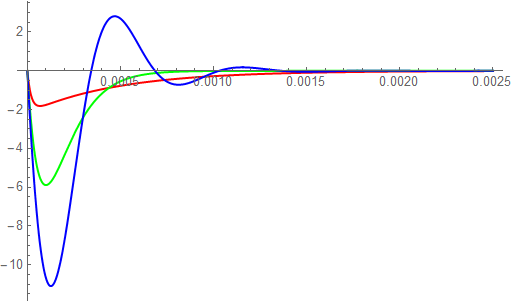
\includegraphics[scale=0.7]{respuestatemporal1}
	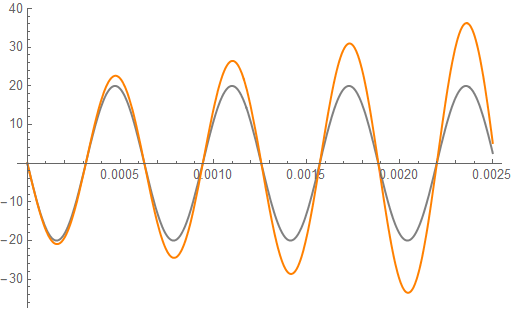
\includegraphics[scale=0.7]{respuestatemporal2}
	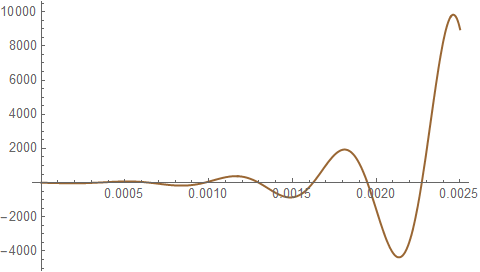
\includegraphics[scale=0.8]{respuestatemporal3}
\end{center}	
\begin{center}
	\begin{tabular}{|c|c|c|}
	\hline 
	Color&$R_{2}$ & Tipo de Respuesta \\ 
	\hline 
	\hline 
	Rojo&500 & Criticamente Amortiguada \\ 
	\hline 
	Verde&800 & Subamortiguada \\ 
	\hline 
	Azul&920 & Sobreamortiguada \\ 
	\hline  
	Gris&1000 &Oscilatoria \\ 
	\hline 
	Naranja&1005&Inestable  \\ 
	\hline 
	Marrón&1050&Inestable  \\
	\hline
\end{tabular} 
\end{center}



%V_{o(t)}=\frac{d}{\sqrt{b}}\left[e^{\left(-a-\dfrac{\sqrt{b}}{c}\right)t}-e^{\left(-a+\dfrac{\sqrt{b}}{c}\right)t}\right]
%En donde: 
%a=\frac{R_{1}}{2 \text{L}}+\frac{R_{2} R_{b}}{2 \text{L} R_{a}}+\frac{R_{2}}{\text{L}}
%b=(\text{C} R_{1} R_{a} +2 \text{C} R_{2} R_{a} +\text{C} R_{2} R_{b})^2-4 \text{C} \text{L} R_{a}^2
%c=2 \text{L} \text{C} R_{a}
%d= (R_{a}+R_{b})R_{2}C
%R=1000
%L=10mH
%C=1u F
\newpage
\section{Barrido Paramétrico}
Para observar el comportamiento del circuito ante cambios en el valor de la resistencia equivalente se realiza un barrido paramétrico en LTSpice:
\begin{center}
    \begin{circuitikz}[american voltages, american inductors]
	\draw (0,0) node [op amp](amp){U1};
	\draw (amp.-) to [C=1<\micro\farad>] ++(-2,0) to [L=10<\milli\henry>] ++(-2,0) to [R=1<\kilo\ohm>] ++(-2,0) node[ground]{};
	\draw (amp.-) to[short,*-] ++(0,1.5) coordinate (leftR2) to[R=1<\kilo\ohm>] (leftR2 -| amp.out) to[short,-*] (amp.out);
	\draw (amp.out) to [R=1<\kilo\ohm>]++(0,-2) coordinate (rightRa);
	\draw (amp.+) to [short]++(0,-1.51) to [short,-*](rightRa);
	\draw (rightRa) to [R,l=$\{Rb\}$]++(0,-2) node[ground]{};
	\draw (amp.out) to [short,*-o]++(1,0)node [right] {$V_{o(t)}$};
	\node at (-5.8,-2.5){.tran 20ms uic};
	\node at (-3.8,-3){.step param Rb list 500 800 920 1k 1005 };	
	\node at (-5.6,-2){.ic V(N001) = 1};
	\node at (-5.6,-1.5){.ic V(N004) = 0};
	\draw (amp.up) --++(0,0.1) node[vcc]{12\,\textnormal{V}};
	\draw (amp.down) --++(0,-0.1) node[vee]{-12\,\textnormal{V}};
\end{circuitikz}
\end{center}

Es necesario configurar la condición inicial del capacitor con una tensión de 1V, usando la etiqueta $\textsc{.IC}$ se puede establecer la condicion inicial de tensión en un nodo. Se obtuvieron las siguientes respuestas:

\begin{center}
    \begin{tikzpicture}[
        ]
        \begin{axis}[
        xlabel=$Tiempo$, ylabel=$V_{o(t)}$, grid=major,legend entries={$500\Omega$,$800\Omega$,$920\Omega$}
        ]
        \addplot[color=red,
        select coords between index={1}{400},
        filter discard warning=false, unbounded coords=discard
        ] table [x index=0, y index=1]{r500.txt};
        \addplot[color=green,
        select coords between index={1}{400},
        filter discard warning=false, unbounded coords=discard
        ] table [x index=0, y index=1]{r800.txt};
        \addplot[color=blue,
        select coords between index={1}{400},
        filter discard warning=false, unbounded coords=discard
        ] table [x index=0, y index=1]{r920.txt};
    \end{axis}
    \end{tikzpicture}
\end{center}
En donde las diferentes respuestas están diferenciadas por trazos de diferentes colores:
\begin{itemize}
	\item Rojo: Respuesta criticamente amortiguada.
	\item Verde: Respuesta subamortiguada.
	\item Azul: Respuesta sobreamortiguada.
\end{itemize}
\begin{center}
    \begin{tikzpicture}[
        ]
        \begin{axis}[
        xlabel=$Tiempo$, ylabel=$V_{o(t)}$, grid=major,legend entries={$1000\Omega$,$1005\Omega$}
        ]
        \addplot[color=gray,
        select coords between index={1}{400},
        filter discard warning=false, unbounded coords=discard
        ] table [x index=0, y index=1]{r1000.txt};
        \addplot[color=orange,
        select coords between index={1}{400},
        filter discard warning=false, unbounded coords=discard
        ] table [x index=0, y index=1]{r1005.txt};
    \end{axis}
    \end{tikzpicture}
\end{center}
\begin{itemize}
	\item Gris: Respuesta oscilatoria.
	\item Naranja: Respuesta inestable.
\end{itemize}

%Se puede observar que el trazo verde representa una respuesta criticamente amortiguada, el trazo azul una respuesta sobreamortiguada, el trazo rojo un oscilador y el trazo negro una respuesta inestable. 
\section{Conclusión}

El sistema tiene un comportamiento oscilatorio cuando no existe amortiguamiento, es decir el valor de $\xi$ es nulo. Que un sistema tenga amortiguamiento significa que la energía se está disipando y luego de un determinado tiempo llegará a un equilibrio estable.

Al realizar el modelo matemático se debe tener en cuenta de no utilizar ecuaciones integro-diferenciales ya que al aplicarle la transformada de Laplace se pierde información del sistema.
  
Se pudo graficar exitosamente en Mathematica la tensión de salida para diferentes tipos de respuesta.
\end{document} 
